
\documentclass[10pt]{article}
\usepackage[T1]{fontenc}
\usepackage{amssymb}
\usepackage{amsmath}
\usepackage{graphicx}
\usepackage{algpseudocode}
\usepackage{algorithm}



\usepackage{tikz}
\usetikzlibrary{arrows}
\usepackage{subfigure}
\usepackage{stackrel}
\usepackage{blindtext}

\usepackage{biblatex}
\addbibresource{library.bib}

\oddsidemargin=0.15in
\evensidemargin=0.15in
\topmargin=-.5in
\textheight=9in
\textwidth=6.25in

\usepackage[colorlinks=true,breaklinks,pdfpagemode=none,linkcolor=blue,citecolor=blue]{hyperref}

\usepackage{enumerate}
\usepackage{enumitem}
\setlist{itemsep=-1mm}



%\usepackage[usenames,dvipsnames]{pstricks}
%\usepackage{epsfig}
\usepackage{amsmath,amsfonts,amssymb,bm}
%\usepackage{pst-grad} % For gradients
%\usepackage{pst-plot} % For axes


%% Environment definitions (add your own here)

\newtheorem{theorem}{Theorem}
\newtheorem{corollary}[theorem]{Corollary}
\newtheorem{lemma}[theorem]{Lemma}
\newtheorem{observation}[theorem]{Observation}
\newtheorem{proposition}[theorem]{Proposition}
\newtheorem{definition}[theorem]{Definition}
\newtheorem{claim}[theorem]{Claim}
\newtheorem{fact}[theorem]{Fact}

\newenvironment{proof}{\noindent{\bf Proof}\hspace*{1em}}{\qed\bigskip}

%% New commands (add your own here)

\newcommand{\eps}{\varepsilon}
\newcommand{\bbR}{\mathbb{R}}
\newcommand{\hv}{\hat{v}}
\newcommand{\hL}{\hat{L}}
\newcommand{\hlambda}{\hat{\lambda}}
\newcommand{\homega}{\hat{\omega}}
\newcommand{\hp}{\hat{p}}
\newcommand{\hW}{\hat{W}}
\newcommand{\cK}{\mathcal{K}}
\newcommand{\qed}{\rule{7pt}{7pt}}
\newcommand{\cF}{\mathcal{F}}


\begin{document}

   \noindent
   \begin{center}

   \hrulefill
   
   \vspace{5pt}
   
   \makebox[\textwidth]{ {\bf Energy Systems Analysis} \hfill  A.D. Smith 2019}
   \vspace{0pt}
   
   {\Large \hfill  Lecture 3. U.S. Energy Sector, Power Generation, and Built Environment}
   \vspace{5pt}
   
  
   \hrulefill
   \end{center}
   
{\color{darkgray}{\center{ \small{      ``We consume electricity, transportation, and heat, not coal, nuclear, or solar power. And we want energy delivered with certain attributes---namely, energy that is inexpensive, dependable, and safe. To the typical American, even to most U.S. companies, the energy choice is not really about the fuel used.''
\\%[3pt]
\rightline{{\rm --- Stephen Ansolabehere in \textit{Cheap and Clean} \cite{Ansolabehere2014-fi}}}}}}}


\section{U.S. Energy Sector}
The \textbf{primary energy} sources in the U.S. are:

\begin{itemize}
    \item fossil fuels (petroleum, natural gas, coal);
    \item uranium (nuclear fuel); 
    \item biomass (plant- and animal-derived fuels); and
    \item water, wind, sun, and geothermal resources;
\end{itemize}


and the use of energy falls into four main sectors (in addition to the electricity generation sector, which itself serves each of the four sectors listed below):

\begin{itemize}
    \item transportation,
    \item industrial, 
    \item commercial, and
    \item residential.
\end{itemize}


You can see the most recent estimates for U.S. energy use, and which sectors it went to, in the famous Sankey diagram published by Lawrence Livermore National Lab \cite{noauthor_undated-zv}, shown in Figure \ref{sankey}. 

Remember from thermodynamics that 100\% efficiency is often not possible, even with theoretically perfect devices (e.g. a Carnot engine), so ``rejected energy'' does not necessarily mean ``wasted energy'' and does not even necessarily correlate to lost available work (inefficiencies). The flows from left to right on this diagram represent many types of thermodynamic processes and devices: combustion, nuclear fusion, heat engines, electrochemical energy conversion, electromechanical energy conversion, and many more. They often include combinations of multiple energy conversion processes, for example:  natural gas combustion (blue box on the left, Fig. \ref{sankey}) to create electric power (orange box, Fig. \ref{sankey}) to charge an electric car battery and eventually run its motor for personal transport (pink box on the bottom right, Fig. \ref{sankey}).

            \begin{figure}[h]
      %      \centering
            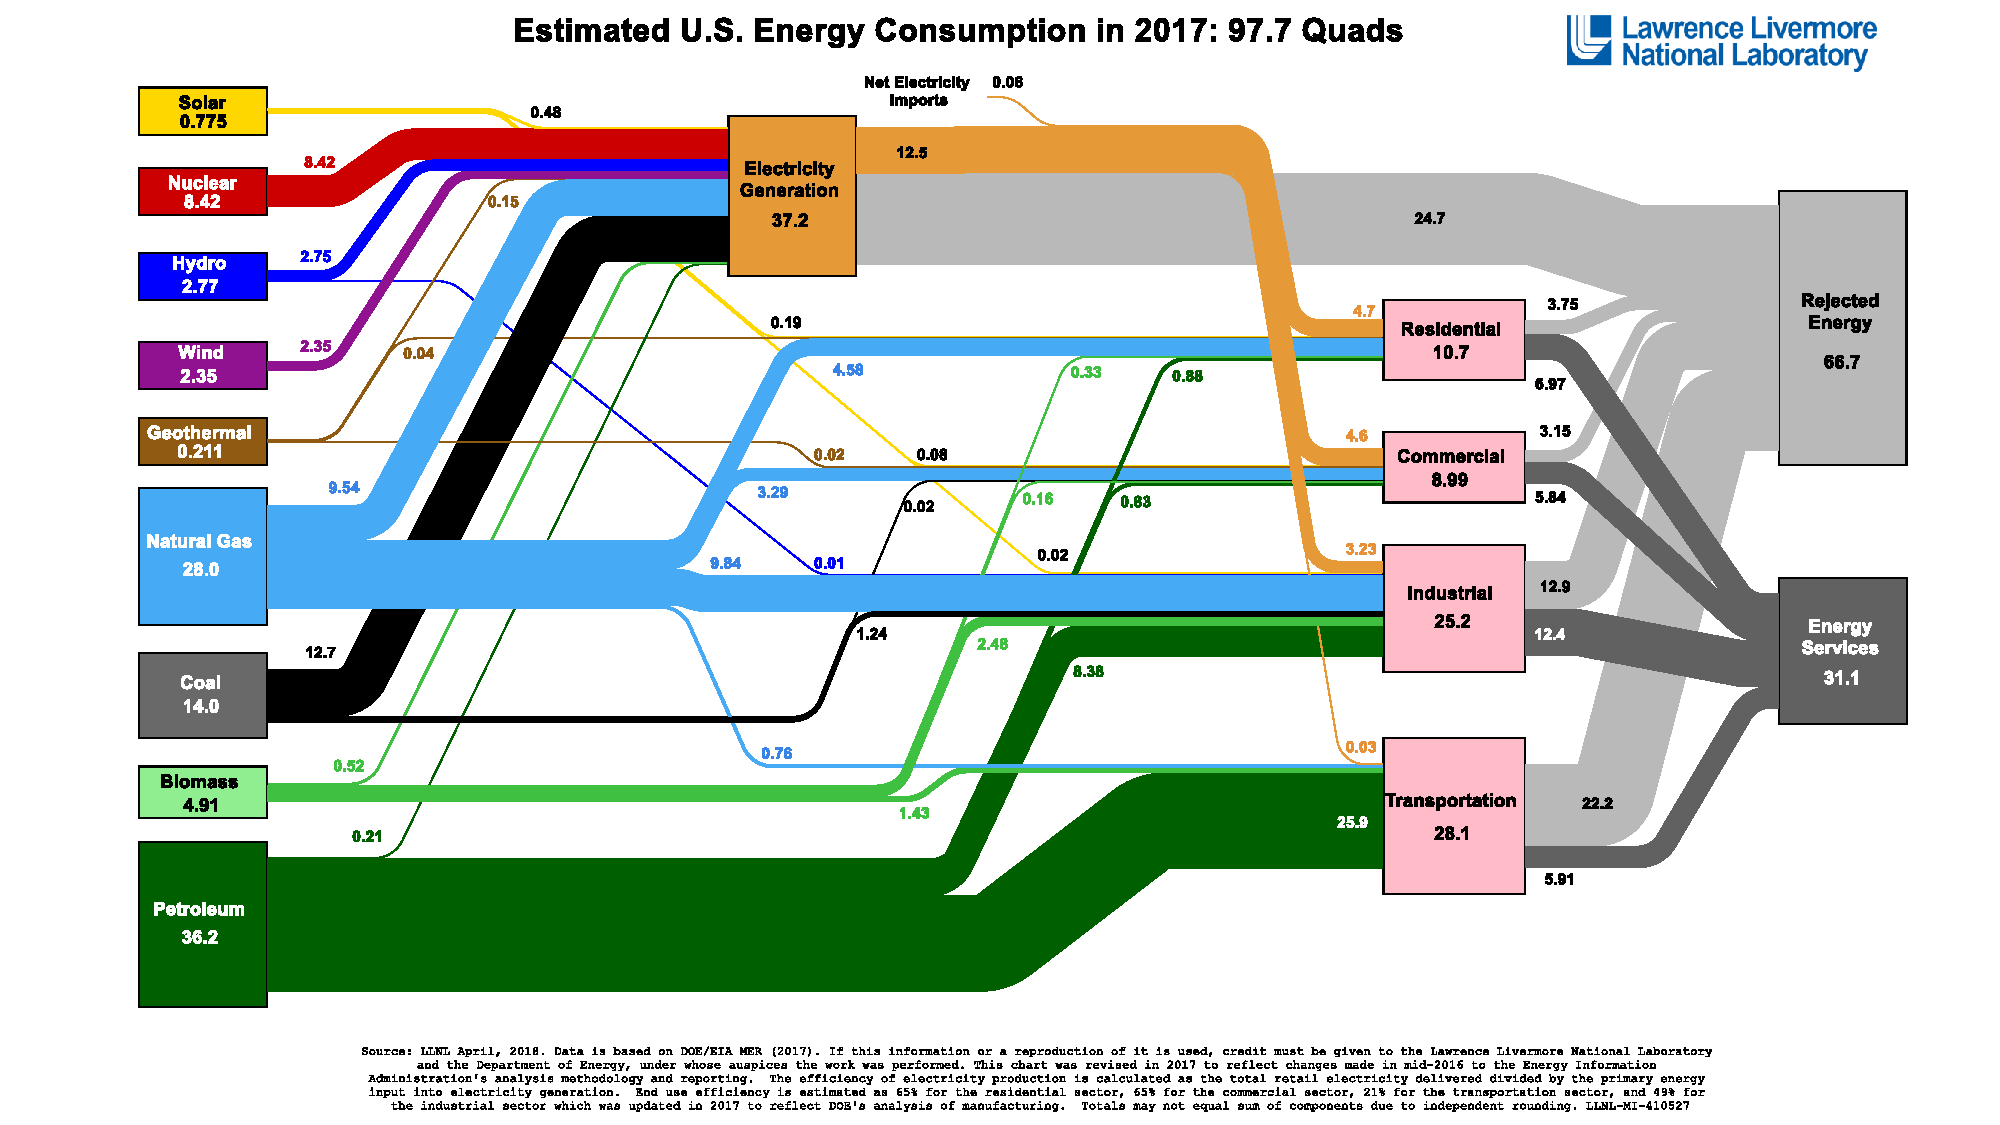
\includegraphics[width=7in]{extras03/2017_United-States_Energy.pdf}
            \caption{U.S. energy flow chart for 2017 from LLNL \cite{noauthor_undated-zv}}
            \label{sankey}
            \end{figure}



\section{Power Generation}

{\color{darkgray}{\center{ \small{      ``America isn't making electricity the way it did two decades ago.''
\\%[3pt]
\rightline{{\rm --- Nadja Popovich in the New York Times \cite{Popovich2018}}}}}}}

\smallskip

Electric power produced in the U.S. still comes mostly from natural gas, coal, and nuclear plants. 

In general, we can categorize these electricity generation facilities as

\begin{itemize}
    \item \textbf{thermoelectric} power generation (coal-fired, gas-fired, and nuclear),
    \item \textbf{hydroelectric} power generation, and
    \item other renewable/alternative forms of power generation (solar PV, solar thermal, wind, biomass, and others).
\end{itemize}

Hydropower, wind, and solar are the next largest contributors to U.S. electricity generation, though relatively small compared to gas, coal, and nuclear. What is \textit{not} reflected in Figure \ref{sankey} (2017) is that natural gas was estimated to have contributed to more electricity generation than coal as of last year (2018). The use of natural gas has increased somewhat steadily since 2013, while coal plants are being retired and little to no new coal-fired generation is coming online. The makeup of generators serving the grid is changing rapidly in recent years. Explore interactive graphs from the U.S. Energy Information Administration (EIA) for yourself at \url{https://www.eia.gov/electricity/data/browser/}.

\subsection{International}

Worldwide, most electricity generation comes from from coal, with natural gas gaining very quickly and poised to overtake coal soon. Other significant power sources are: hydro, wind, nuclear, and solar PV \cite{noauthor_undated-ge}. Explore interactive graphs from the International Energy Agency (IEA) for yourself at \url{https://www.iea.org/weo/}.

A large portion of the power generated in the world comes from the Organisation for Economic Co-operation and Development (\textbf{OECD}) countries (over 10,000 TWh in 2015 \cite{noauthor_undated-gz}), which include the U.S., Canada, and Mexico; the United Kingdom; many EU member states (e.g.  France, Germany, Italy, Switzerland); Australia and New Zealand; Japan and Korea \cite{noauthor_undated-yg}. China alone forms the next largest portion of worldwide power generation (almost 6,000 TWh in 2015 \cite{noauthor_undated-gz}).


\subsection{Utah}

From the recent article ``How does your state make electricity?'' \cite{Popovich2018}:

\begin{quote}

The majority of electricity produced in Utah comes from coal, but coal's share has declined over the last several years as natural gas has increased.

The state produces more energy than it consumes and sends the surplus to nearby states like California. At least one Utah power plant \cite{Linthicum2013} is switching from burning coal to natural gas to comply with California's stricter environmental regulations.

Solar power grew to become the largest renewable generation source in the state in 2016 \cite{brightfuture} and expanded its share again last year. Utah has set a goal for utilities to get 20 percent of the electricity they sell from renewable sources by 2025 \cite{noauthor_undated-xb}.

\end{quote}

Note that the second paragraph describes Utah as a \textbf{net exporter} of electrical power.


\subsection{Electrical transmission \& distribution}

The electrical grid is a complex system-of-systems that comprises physical assets, economic systems, and coordinated networks for communications and operations. It's worth an entire course in and of itself; we have several excellent offerings available through the Department of Electrical \& Computer Engineering. You should view the infographic and brief web page at \url{https://www.energy.gov/articles/infographic-understanding-grid} to familiarize yourself with the big picture if you have not had exposure to the structure and workings of `the grid' before.

There are a few key divisions within the electricity sector as electrical power makes its way to the end user: 

\begin{itemize}
    \item \textbf{generators} (as we have described in this section up to this point);
    \item \textbf{transmission} lines and equipment (high voltage), large and tall structures that move high quantities of power over long distances; and
    \item \textbf{distribution} lines and equipment (lower voltage), usually closer to the ground (and in some places, below ground), that move smaller quantities of power to (or close to) the end user.
\end{itemize}

There are three main transmission networks across the U.S.: \begin{itemize}
\item Western Interconnection (including Utah),
\item Eastern Interconnection, and
\item Electric Reliability Council of Texas (ERCOT).
\end{itemize}

The state of Hawaii is, as you might imagine, on its own, with unique geographical challenges  \cite{noauthor_undated-wl}.

\section{Built Environment}

Buildings and facilities are typically divided into three main sectors: 

\begin{itemize}
    \item industrial, 
    \item commercial, and
    \item residential.
\end{itemize}

The EIA publishes estimates of energy use in the U.S. in three major survey efforts:

\begin{itemize}
    \item Manufacturing Energy Consumption Survey (MECS) \cite{noauthor_undated-dy}
    \item Commercial Building Energy Consumption Survey (CBECS) \cite{noauthor_undated-va}
    \item Residential Energy Consumption Survey (RECS) \cite{noauthor_undated-wv}
\end{itemize}

These surveys provide thorough and detailed estimates based on extensive data collection and processing, but new releases are years apart and therefore they may not have the most up-to-date information.

In this class, we will focus on commercial and residential buildings when we study energy use in the built environment. We all interact with both commercial and residential buildings daily, unless we are fortunate enough to be out on a multi-day camping trip or unfortunate enough to be without a home or shelter.
The most recent estimate from the EIA states that `` In 2017, about 39\% (or about 38 quadrillion British thermal units [quads]) of total U.S. energy consumption was consumed by the residential and commercial sectors.'' \cite{noauthor_undated-ow}:


%%% Add from Ch. 2\cite{Ansolabehere2014-fi}

% license
\bigskip

\noindent
\texttt{\footnotesize RESTRICTED PUBLIC LICENSE --- READ BEFORE SHARING. This is a draft version made available by Amanda D. Smith under a Creative Commons Attribution-NonCommercial-ShareAlike license. 
\href{https://creativecommons.org/licenses/by-nc-sa/4.0/}{CC BY-NC-SA 4.0}}

% references
\newpage
\printbibliography

\end{document}